\chapter{Depth-of-Field}
As discussed in chapter \ref{ch:background} virtual cameras are able to take perfect color samples from every angle and thus create an image with infinite \gls{dof}.
However without expensive operations, like the simulation of a lens with path tracing, a virtual camera is only able to create perfect images.
As such the difficulty in simulating depth of field in real-time lies in combining images with infinite \gls{dof} into good approximation of real camera images.
The ideal method would be able to satisfy the following criteria:
\begin{itemize}
    \item Specification of a point-spread-function
    \item Per-pixel blur level control
    \item Lack of intensity leakage
    \item Lack of depth discontinuity artefacts
    \item Simulation of partial occlusion
    \item High performance
\end{itemize}

\todo{Explain intensity leakage, discontinuity artefacts and partial occlusion}

\section{Accumulation buffers}
The earliest method to generate a depth-of-field effect using traditional rasterization hardware was presented by Haeberli and Akeley. \cite{Haeberli.1990}
Their method introduces the use of an accumulation buffer to the rendering pipeline to simulate multiple effects, including motion blur and \gls{dof}.
The accumulation buffer is a region of memory used by the rendering hardware to accumulate and average the results of multiple rendering passes.
To simulate a depth-of-field effect the following steps are iterated:
\begin{enumerate}
    \item \textbf{Jittering:} The camera position is slightly disturbed. Commonly done by offsetting the principal point of the camera, but keeping the camera pointed at the same point in the scene
    \item \textbf{Rendering:} An image is created using the traditional rasterization pipeline
    \item \textbf{Accumulation:} The rendered image is added to the accumulation buffer.
\end{enumerate}
The jittering of the camera simulates the size of the individual image pixels of a real image sensor.
The images are then averaged to approximate the integration of all light paths hitting a sensor pixel.
As such out of focus objects will have varying positions in the rendered images and thus are spread out over their \gls{coc} in the final image.
This method therefore converges on the correct solution and does not suffer from the image artefacts mentioned earlier.

\begin{wrapfigure}{R}{0.4\linewidth}
\begin{center}
    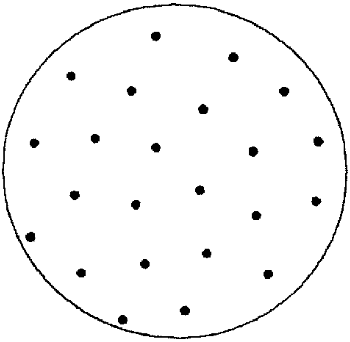
\includegraphics[width=0.38\textwidth]{images/sample-locations.png}
\end{center}
\caption{Position of sample location used to sample the aperture of the camera lens. \cite{Haeberli.1990}}
\label{fig:sample-pos}
\end{wrapfigure}

The specific approach to jittering the camera is subject to the individual implementation, but should move the camera parallel to the image plane.
Sampling points in a circular area may be used to simulate a circular aperture, but a hexagonal or octagonal sampling shape may be preferred for mechanical apertures.
Similarly the distribution of points may be adjusted achieve a specific \gls{psf}.
As such this approach great artistic flexibility.

To hide the individual frames a minimum density of samples must be taken to sufficiently cover the biggest \gls{coc} present in the image.
As such the amount of work needed to get acceptable results scales linearly with the \textbf{area} of the biggest \gls{coc} created by the scene.
Acceptable results are typically achieved with a single pass per 4 pixel area of the \gls{coc}.
This still results in 50 passes at a \gls{coc} with a 8 pixel radius. \cite{Demers.2005}
Thanks to the use of a traditional rasterization pipeline this method is often faster than ray-traced approaches.
However the high increase in the rendering workload excludes its use in all but the most CPU-bound real-time rendering workloads or as reference images.

\section{Single-Layer approaches}
To improve on the performance of accumulation buffers, several techniques have been developed, that limit themselves to a single rendering pass.
In addition to the color information in the frame buffer, all these techniques store the depth of each pixel in a separate z-buffer.
The main way the following methods differ is in their use of the given data to create the final image.
Due to the limitation on the information provided, all of the following methods exhibit some artifacts, that are accepted for the higher performance they offer.

The single-layer approaches can be categorized into two sub-categories based on the direction of how the final color for each pixel is calculated.

\subsection{Scattering methods}
The first method to generate depth of field, commonly referred to as \textit{splatting}, or \textit{forward-mapped z-buffer \gls{dof}} was introduced by Potmesil et al. \cite{Potmesil.1981}
It uses the fact that the image of pinhole camera stores the light intensity for \textbf{most} directions that hit the sensor.
With the additional information of the depth we can calculate the \gls{coc} of each light ray.
To efficiently calculate the final color of a pixel, a sprite with the calculated \gls{coc} size is placed at its position.
The color of the sprite is taken from the original pixel while its alpha value is inversely proportional to the size of the \gls{coc}.
As with the use of accumulation buffers the shape an color of the sprite can be modified to simulate a specific \gls{psf}.
The sprite is then placed at the original distance and second rendering pass is used to generate the final image.

The resulting image is a very close approximation of an image generated by the accumulation buffer method.
The main visual imperfection created by this method is the lack of partial occlusion.
This is barely noticeable in static scenes, but causes bright objects to suddenly appear when coming into view behind other objects.
As this method relies on the interaction of transparent sprites, we must sort a sprite for each pixel.
This log-linear time complexity in regard to the resolution is the main drawback of this method.
While highly interactive application such as video games may not find this performance acceptable, the high quality make it an attractive option for providing previews of renders.\cite{Demers.2005}

\subsection{Gathering methods}
Each pixel is blurred according to distance from focus plane.
Can be implemented by LERPing between mip-maps of image.
To lessen interpolation artefacts of mip-maps a gaussian filter or other PSF can be used.
The depth map may also be mip-mapped or blurred to lessen the effects of depth discontinuities.
\cite{Gilham.2007}, \cite{Hammon.2008},\cite{Zhou.2007} or \cite{Lee.2009}

\section{Multi-Layer approaches}
The multi-layer approaches have been developed to address the problem of intensity leakage and the lack of partial occlusion.
The rendered pin-hole image is decomposed into several sub-images each representing a layer in the scene.
Pixel at the edges are lerped across two sub-images to mask transition between layers, especially on objects that span across layers.
The partial occlusion is addressed by extrapolating the occluded pixels in a sub-layer.
The image quality is often better than single-layer approaches, but they suffer from many texture lookups and therefore reduced performance.

\cite{Kraus.2007}

